\documentclass[10pt,a4paper]{article}
\usepackage[margin=1.25in]{geometry}
\usepackage{fancyhdr} % fancy header
\pagestyle{fancy} % so fancy
\usepackage[round]{natbib} % bibliography
\usepackage{graphicx} % for importing graphics / figures
\usepackage{booktabs} % publication-worthy tables
\usepackage{multirow}
\usepackage{adjustbox} % makes tables fit nicely on the pag
\usepackage{amsmath}
\usepackage{algorithm}
\usepackage[noend]{algpseudocode}

\lhead{Josh MEYER}
\rhead{Dissertation Prospectus}
\cfoot{} %% make empty to get rid of the page number %% \cfoot{Page \thepage}
\renewcommand{\footrulewidth}{0.4pt} %% this puts a fancy line at the footer


\begin{document}


\section{Goals \& Import of Dissertation}

The main goal of this dissertation is to develop training methods for neural networks which lead to better classification of data from unseen conditions. In particular, this work focuses on small data sets, where traditional neural net training leads to overfitting.

When training a statistical classifier on a small data set, the researcher must take extra precautions to avoid overfitting. A powerful model (such as a deep neural network) will easily achieve 100\% classification accuracy on a small training dataset, because the model learns ``useful'' noise in its parameters. However, that ``useful'' noise is specific to the training data, and will not generalize to a new dataset. For example, deep neural network training to classify images of cats and dogs may learn to associate teeth with dogs, if some of the dogs have their mouths open. This kind of random chance occurs more often with small datasets, which means the smaller the dataset, the worse the generalization of the model. If this cat vs dog classifier gets a new picture of a cat with its mouth open, it may be very well classified as a dog.

Likewise, in speech recognition we must be careful with small datasets, so that our acoustic models don't learn ``useful'' noise during training. The sources of this noise in speech recognition stem from background conditions (busy streets vs quiet room), the person doing the talking (old woman vs young boy), or an extreme example is the language itself. A small dataset of speech from an audiobook will produce an acoustic model which fails miserably on speech from a noisy car. The most common approach to combat this problem is to collect a new, bigger dataset from the target condition. However, if we want speech recognition that is truly human-like, we need to develop training techniques which lead to better generalization.

This dissertation investigates training techniques for acoustic modelling on small datasets. To determine the generalizability of the resulting models, the training and testing datasets are sampled from very different recording conditions. The unseen testing data conditions are (1) \texttt{new noise}, (2) a \texttt{new speaker}, or (3) a \texttt{new language}.


Using the framework of Multi-Task Learning, I train a single neural net to classify a small dataset with several tasks, encouraging the hidden layers to learn generic, useful represetations of the data. This is accomplished without any explicit adaptation of model parameters or data transformations.

\begin{enumerate}
  
\item For the \texttt{Noise} condition, I train on clean audio and test on noisy audio.
\item For the \texttt{Speaker} condition, I train on a set of speakers, and I test on an unseen speaker.
\item For the \texttt{Language} condition, I train on (mostly) English, and I test exclusively on Kyrgyz.
\end{enumerate}
    
My approach is innovative because it doesn't require massive data sets, as some other popular reseach labs have relied on (Google, Firefox, Baidu, Microsoft, etc), and it doesn't require tuning the net to the new dataset (e.g. fMLLR). Further more, my approach is not specific to any one dataset, and it can be used to train any neural net (not just for speech recognition).

MTL training for neural nets works by training a set of hidden layers to perform multiple tasks (multiple output layers). Here is an example of MTL architecture for an acoustic model from Heigold 2013.

\begin{center}

\includegraphics[width=.85\textwidth,keepaspectratio]{figs/heigold-2013-dnn-c.png}
\end{center}

This is the architecture that will be used in my dissertation. The number of input nodes on my neural nets corresponds to the dimensionality of audio features, and the number of nodes on each output layer corresponds to the number of phonemes (i.e. monophones or triphones) I've defined for the language.

During training all \texttt{Tasks} are trained in unison, but during testing only one \texttt{Task} is used. The only benefit from these extra tasks comes from the training phase, and their influence on the shared hidden layers.






\newpage

\section{Overview of Speech Recognition}

All research exists in some historical context, answering pressing questions of the times, making use of and reacting to existing technologies. ASR research is a fine example of a field which has grown in directions defined by either military, academic, or commercial incentives. Early work on ASR reflected the needs of telecommunications companies. Then came a wave of interest from the US Department of Defense, and most recently the four tech giants (Google, Amazon, Facebook, and Apple) have set the bar for what is classified as meaningful research. While all these initiators pushed researchers in different directions, they all share one common goal: to make ASR more human-like.

This section contains the training and testing procedures for standard automatic speech recognition (ASR) pipelines. The overview will provide the reader with a technical grounding in ASR, so that the rest of the dissertation will have some point of reference. 

\subsection{1952: Isolated Word Systems: Bell Labs}
Most of the early work on ASR in the 50's and 60's focused on isolated word, speaker-dependent speech recognition. This line of work was lead by research labs in telecommunications companies like Bell Labs and NEC Corporation (a Japanese technology giant), and also academic labs like MIT Lincoln Labs. (TYPICAL XXX)

Given the interests of the researchers, the typical use case was a single adult male carefully reading off single digits [0-9] into a microphone. One of the very first demonstrations reported accuracy rates of up to 99\% on isolated digit recognition \cite{davis1952automatic}. This system relied on the formant frequencies of speech to recognize entire words. That is, there was no concept of syllables or consonants or vowels in these systems. The word was treated as a single unit, and during classification all words were compared to each other to find the best match.

This work, along with most others of this time period, relied on a template-matching framework to classify spoken words. An exmplar of each word was saved to disk (for each speaker ideally), and when a user spoke a new, unknown word into the microphone, the computer compared that audio with all the examplars it had on file for that speaker. The closest match was returned back, and when recognizing a set of ten digits, this worked surprisingly well. 

The Bell Labs system worked in the following way:

\begin{enumerate}
\item FEATURE EXTRACTION
  \begin{enumerate}
  \item two frequency ranges of the audio are extracted, which roughly correlate to the first two formants of speech
  \item these two formants are plotted on an x-y axis in time
  \end{enumerate}
  
\item TEMPLATE MATCHING
  \begin{enumerate}
  \item the 2-D x-y plot from new audio is compared to each of 10 examplars on file, and closest is returned
  \end{enumerate}
\end{enumerate}


An example set of templates (from the original Bell Labs paper) is show below:


\begin{center}
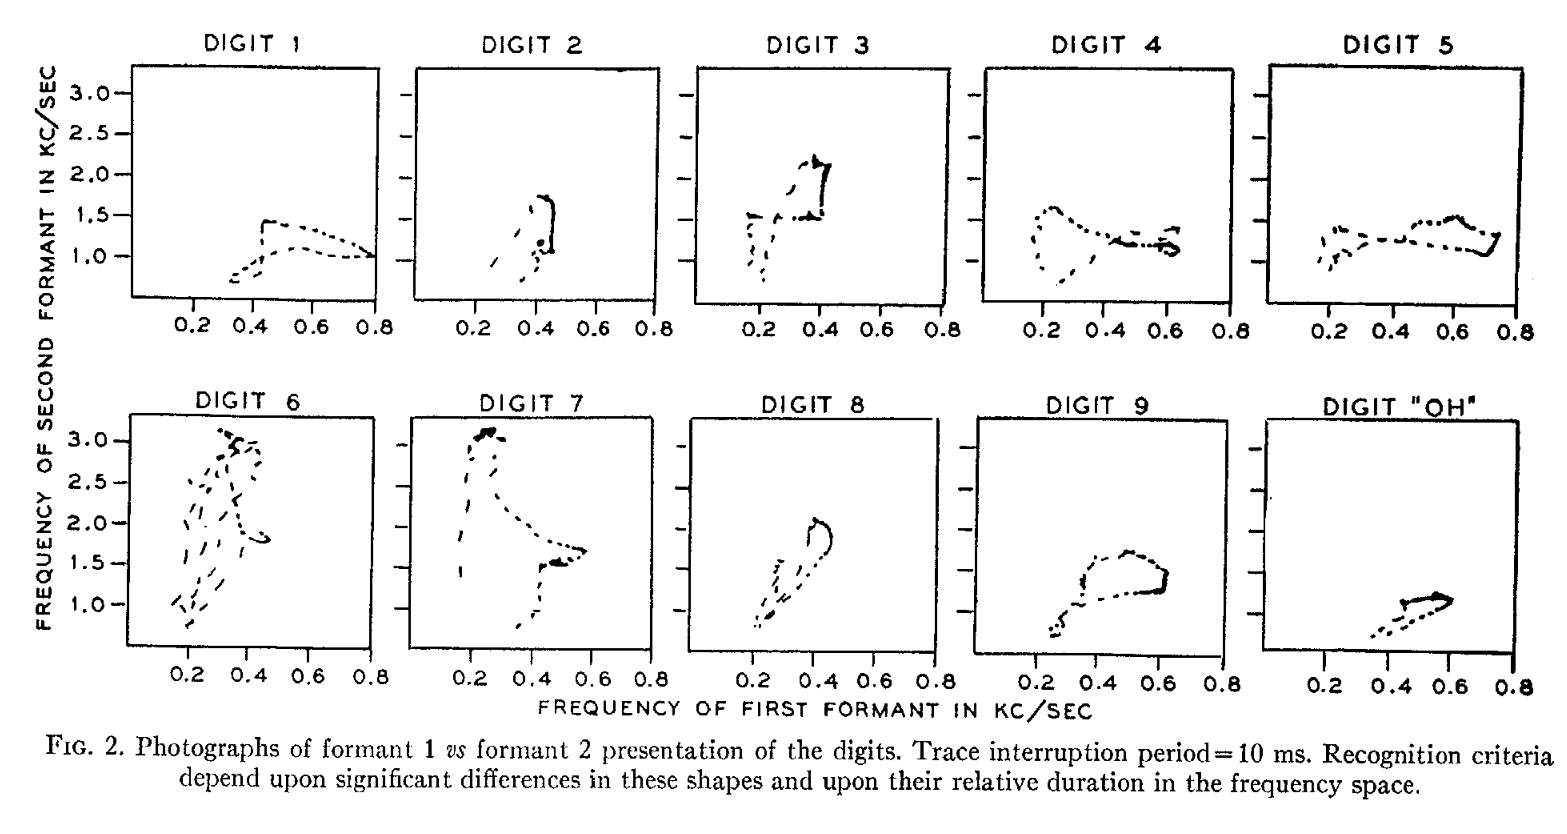
\includegraphics[width=.9\textwidth,keepaspectratio]{figs/digits.png}
\end{center}


It may sound like speech recognition research was off to a great start with Word Error Rates (WER) so low, but in truth the approach taken in much of this early work could not be extended further. These approaches relied on acoustic properties of vowels in a pattern-matching scheme which requires a representation of each word in the vocabulary saved on disk.

If the system were to recognize 1000 words instead of just 10, the time needed to compare new input to each of the 1000 examplars would be prohibitive. Additionally, the space on disk would increase with every additional word. A more serious limitation is the approach of whole-word template-matching via formant frequencies. Two words with similar consonants and identical vowels (eg. `dog' vs `dock') would be nearly indistinguishable for the system.

\subsection{1971: Constrained Sentence Recognition: ARPA}

 Speech research soon was boosted into full gear when in 1971, the Advanced Research Program Agency (ARPA) of the US Department of Defense launched the 5-year Spoken Understanding Research (SUR) program. The goal of the program was to ``obtain a breakthrough in speech understanding capability that could then be used toward the development of practical man-machine communication systems.'' \cite{klatt1977} ARPA wanted something that Airforce pilots could control with their voice while their hands were busy steering. The SUR program spurred various papers from four main research groups (TYPICAL SUR PAPERS). Probably the most significant result of the ARPA project was James Baker's 1975 dissertation at CMU, which firmly established the import of the Hidden Markov Model in ASR \cite{bakerDissertation1975}.


 The contestants were given the task of creating a system which could recognize simple sentences from a vocabulary of 1000 words with a 10\% WER in reasonable time. In order to make a recognizer that could handle sentences instead of isolated words, where the length of that string was unknown to the system, major overhauls of the Isolated Word system were needed.

First of all, it was clear that storing an exemplar of each word on disk is not an option with continuous speech systems. In addition to the nearly impossible task of discovering word boundaries from raw audio, the decoding speed would be horrendous if the words were found. The machine would have to compare each word to each of the 1,000 candidate words on disk. Furthermore, the space used on disk would be prohibitive, not to mention the time needed by the user to record every word during speaker enrollment. Modeling whole words became an obvious bottleneck to recognition of continuous speech. As such, speech needed to be modeled at a level lower than words themselves, and the phoneme became an obvious candidate.

The phoneme is the smallest meaningful speech sound. Every language has a finite set of phonemes, and with this finite set of phonemes all words are created. Typically languages don't have more than 50 phonemes, and that number will not increase with vocabulary or grammar complexity. Where simple systems had hard limits of 100 or 1000 words, with only 50 discrete phonemes there is no upper limit to the number of words a system can recognize.

All of the teams in the ARPA project used the phoneme as the unit for modelling speech, but the team at Carnegie Mellon showed best promise with their `Harpy' system. \cite{juang2005automatic} Like in Isolated Word Recognitions, all teams used some kind of template matching, but with phoneme templates instead of word templates.

The Harpy system decoded a new utterance in the following way:

\begin{enumerate}
\item FEATURE EXTRACTION
  \begin{enumerate}
  \item process audio with 5kHz low-pass filter and sample to 10k samples per second 
  \item extract linear prediction coefficients in 10-ms frames with a 10-ms shift
  \item group together similar, adjacent acoustic segments
  \end{enumerate}
  
\item GRAPH CONSTRUCTION
  \begin{enumerate}
  \item a set of 98 phonemes (and diphones) defined by expert
  \item pronunciations for all words defined
  \item pronunciations of all accepted sentences in the grammar compiled into one graph (15,000 states with self-loops)
  \end{enumerate}

\item DECODING
  \begin{enumerate}
  \item incoming audio segments compared against 98 templates
  \item best path (with beam search) followed
  \end{enumerate}
\end{enumerate}

An example of what a decoding graph in Harpy might look like is the following (klatt 1977):


\begin{center}
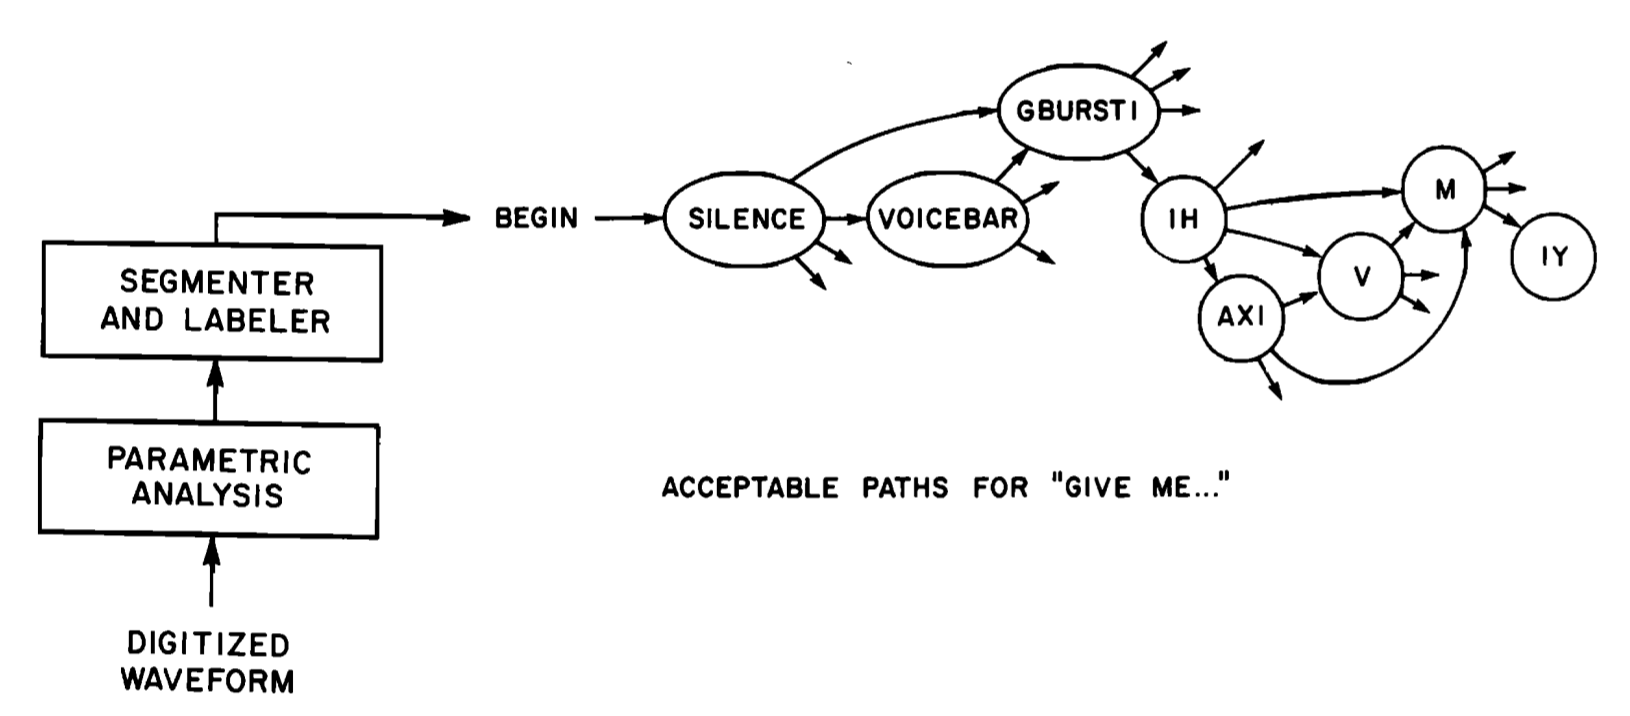
\includegraphics[width=.9\textwidth,keepaspectratio]{figs/harpy-graph.png}
\end{center}


Harpy is a speaker-specific system, and the 98 phoneme templates need to be tuned to each speaker. For a new speaker to be enrolled into the system, she must spend about 30 minutes recording example sentences, which are then force-aligned to the graph. This forced-alignment, however, assumes that at least one speaker has already been enrolled, and their 98 phoneme templates are used to align the next speaker's audio.

Given that command and control was the target application, a limited vocabulary and limited grammar was reasonable. The user said one short sentence (from a constrained, finite set), and the decoder compared that sentence to a graph of all possible sentences, and returned the closest match. This assumes the user actually said a sentence in the machine's vocabulary. Each user was trained to work with the machine (learn its grammar), and the machine was trained to work with each user (via enrollment). 

By modern standards, these recognizers were not flexible. However, what these recognizers lacked in flexibility they gained in accuracy. The machine didn't have to consider more than 1,000 words and a simple grammar. Furthermore, there was no real issue of noise conditions, because recording and testing would be both in quiet conditions. There was no worry about microphone robustness or sampling-rate issues, because the creators knew exactly beforehand what hardware the recognizer ran on. All these problems current ASR research faces were unknown to these early researchers, and their approach was simple, and efficient.

This approach worked just fine until users wanted more. Users wanted something more human-like. First of all, training the recognizer to work for every new user was a hassle. We humans don't need to relearn all sounds in our language when we meet someone new, but these machines did. We humans can understand our friends when we're in an echoey factory or in a small room, but these machines couldn't.

Regardless of the successes of the SUR program, ARPA was dissappointed. The best system, Harpy, decoded in about 80x real time. Harpy could not be used in practice, and speeding her up was not a simple task.

In his review of ARPA's Speech Understanding Research Program, (Klatt 1977) concludes that ``all [teams] failed to meet the ARPA goals'', writes a very gloomy prediction on the future of ASR research funding:

\begin{quote}
  ... it is disruptive to send funding oscillations through thr basic research community and to subject science to fads and anti-fads. The danger now is that funds will be less available for the basic science that must be done in the speech analysis area before real further progress is made.
\end{quote}

In addition to problem of speed, flexibility was a greater concern. The kinds of sentences recognized by Harpy were determined by a BNF grammar. This consisted of a set of hand-crafted rules, and was not easily extensible. Such a set of rules has yet to be constructed for the English language, and even in the 1980's, researchers realized waited for such a grammar was not an option. A major shift was about to take place in the ASR world, moving away from template matching and strict grammars to statistical methods. Instead of hard assignments (grammatical or not), a better system would assign a kind of likelihood to the sentence, word, or sound in question.

\subsection{1986: Hidden Markov Models, \& Gaussian Mixtures: Bell Labs}

Juang 1986

``Speech research in the 1980s was characterized by a shift in technology from template based approaches to statistical modeling methods especially the hidden Markov model approach'' (Speech Recognition by Machine: A Review)


\subsection{1994: The Modern GMM-HMM Approach: CMU Sphinx \& HTK}

HTK was the first toolkit to incorporate all of the core components of Modern GMM-HMM speech recognition, but for all intents and purposes, Sphinx and HTK can be seen as parallel toolkits.

While eventually the two toolkits offered the same capabilities by the mid-ninties, the first version of CMU's Sphinx used Vector Quantized codebooks to estimate emission probabilities on HMM states, while HTK began with GMMs in 1994. Regardeless of their differences in performance, HTK's extensive documentation (The HTK Book) became the reference of choice for most speech recognition researchers. The first results of the HTK system were reported as a benchmark on DARPA's Resource Management task in 1992 (Woodland Young 1992).

The standard GMM-HMM pipeline of HTK is outlined below. 

\begin{enumerate}

\item FEATURE EXTRACTION
  
  The toolkit itself is agnostic as to which features are extracted from the audio signal, but the extraction process is standard. This extraction is not unique to HTK, and there is a large literature on different methods of defining audio features.
  
  A common trait of all modern feature extraction in ASR is the following: the signal in its raw form is not condusive to modelling speech, and feature extraction works to make speech-relevant information more available to whatever statistical model we choose.

  Raw audio is simply air pressure measured in time. It is true that speech is transmitted though air via pressure changes, and as such raw audio contains all the information relevant to human speech. However, that same raw audio contains lots of other information which is not relevant to human speech. Background noise is just as prominent as speech in raw audio, and feature extraction helps to prioritize speech over other noise sources.

  For clean speech recorded in a silent audiobooth, feature extraction is still beneficial because speech sounds are differentiated by amplitudes in both the frequency and time domain. Raw audio does not contain direct information about the frequency domain, so it must be deduced.
  The two standard audio feature extraction techniques in HTK (and in ASR in general) are Mel-cepstral coefficients (MFCCs) or perceptual linear prediction (PLPs).

  Overlapping windows are shifted across the audio, from beginning to end, to extract feature vectors. For each timestep, the audio falling inside the window is subjected to a series of transformations which both reduce the dimensionality of the data and highlight speech-specific information. Typically the windows are 25 milliseconds long, and the the shift is 10 milliseconds. In this way, enough time is allowed to capture phonetic information inside one window.

  
\begin{center}
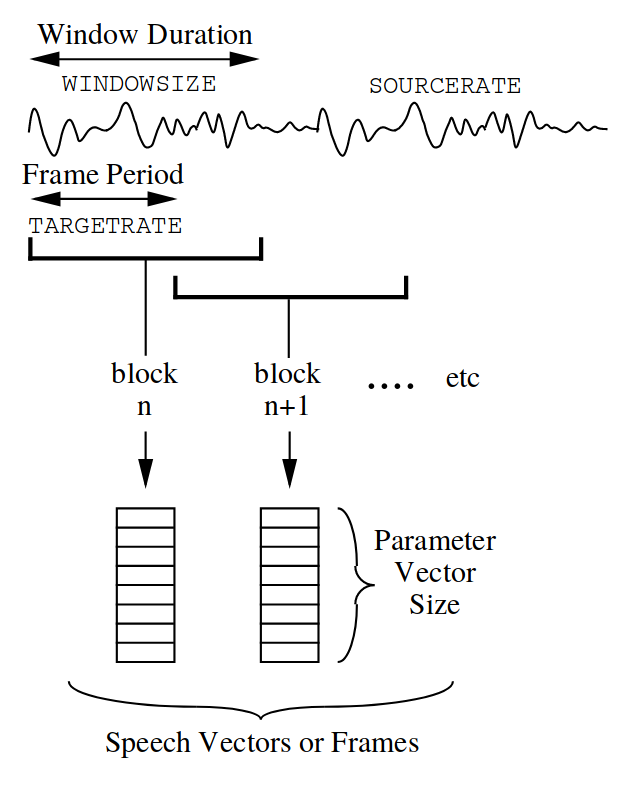
\includegraphics[width=.45\textwidth,keepaspectratio]{figs/htk-feats.png}
\end{center}

Ideally, every feature vector should contain enough information to identify the phoneme which was uttered at that timestep.


\item MONOPHONE TRAINING

  A monophone GMM-HMM acoustic model contains (as the name suggests) one model for one phoneme. For a language with 50 phonemes, a monophone system will have 50 separate GMM-HMMs. However, the number of states in each phoneme's HMM is not specified, and is a matter of researcher discretion. Typically, each monophone HMM will be designated three states as such:

\begin{center}
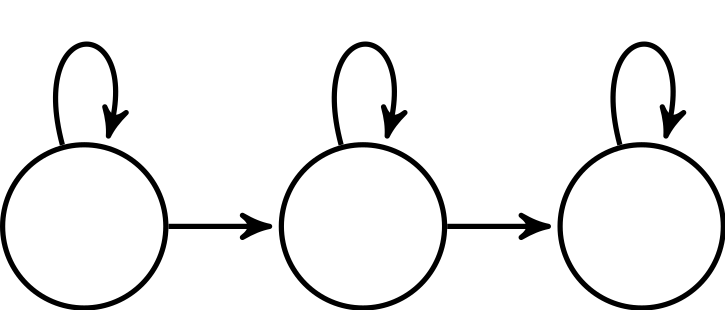
\includegraphics[width=.45\textwidth,keepaspectratio]{figs/3-state-hmm.png}
\end{center}

Given that human speech is a purely left-to-right signal, monophone HMMs are defined to be strictly left-to-right, with the addition of self-loops. The self-loops (as in the Harpy system) nicely model the differences in time which occur in speech. A long, drawn-out vowel will be modeled with the exact same HMM as a short, quick vowel. The longer vowel will just have to pass through more self-loops.

The reason that most GMM-HMMs in speech recognition use three states is the following: neighboring phonemes will blend together, and therefore acoustic features at the edges of sounds may be significantly different from the center of the phoneme. All else being equal, the central state of a monophone should be more consistent than its edges.

Defining a typoglogy for these monophones is not enough to use them in decoding new audio. HMMs are defined by (1) their states, (2) the transitions between those states, (3) the probabilities of transitions between states, and (4) the emission probability of an observation given a state.

So far we have defined how many states we want (three states per phoneme), we have defined the \textit{kinds} of transitions between states (left-to-right or self-loop), and we have defined the shape of the emission probability of each state (a multivariate Gaussian mixture model). However, what this gets us is merely a set of skeleton GMM-HMMs. For these HMMs to be useful, we need to have accurate transition probabilities (s.t. the probability of leaving any non-final state $== 1$) and emissions probabilities (the $\mu, \sigma^2$ for each Gaussian component).

\begin{center}
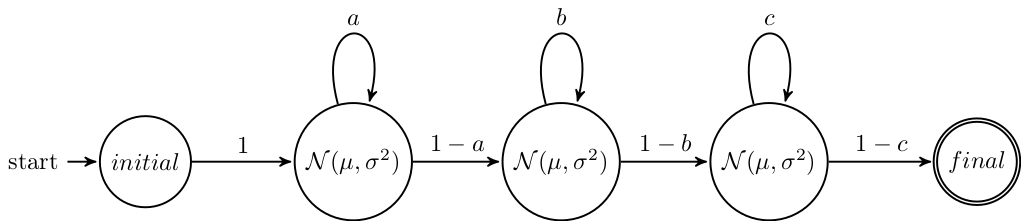
\includegraphics[width=.9\textwidth,keepaspectratio]{figs/skeleton-hmm.png}
\end{center}

One approach to get these numbers would be to down and think really hard about what these numbers should be, filling them in ourselves. We could make self-loops for vowels longer than stop consonants, and we could define the parameters of Gaussians based on some knowledge of acoustic phonetics. However, this is a pretty horrible idea. So instead of trying to guess these values, we use some concepts from machine learning to \textit{learn} them from data.

So, to learn about the acoustics of human speech, we need to collect a lot of it. However, just having access to a huge spoken corpus isn't enough; we need to know which segments of the audio correspond to which states in our GMM-HMMs so that we can update parameters given the appropriate data. While it is certainly possible to align segments of audio to HMM states by hand, it is a very tedious job, and takes about XXX human hours per XXX hour of audio (TIMIT).

A much better approach is to automatically align audio segments (i.e. feature vectors) to HMM states. The algorithms for this alignment have been known since the 1960's (XXX), and are guaranteed to acheive the best model for the given data. This parameter estimation technique is called the Baum-Welch Algorithm, and it falls into the category of Expectation Maximization (EM) algorithms. This is very different from backpropagation with neural nets, which only gets you a local optimum at best.

Given (1) a speech corpus, (2) transcriptions of the speech, and (3) a pronunciation dictionary, we can estimate all the parameters of our GMM-HMMs.

  \begin{enumerate}
  \item Flat-start 

    To successfully train our monophone GMM-HMMs from our speech data, we eventually want to have the entire corpus split into segments which correspond to the states of the HMMs.
    
    To begin training our monophone HMM-GMMs, we need a first guess as to what the sounds may be.

    \begin{center}
      
\includegraphics[width=.9\textwidth,keepaspectratio]{figs/flat-start.png}
    \end{center}

    Flat-start training works in the following way:

    
    \begin{algorithm}
      \caption{Flat Start Alignment}
      \begin{algorithmic}[1]
        \Procedure{Compile Utterance HMMs from Transcripts}{}
        \For{each utterance in corpus}
        \State initialize utterance HMM with start state
        \For{each word in utterance}
        \State lookup pronunciation of word in lexicon
        \For{each phoneme in word}
        \State lookup monophone HMM definition for phoneme
        \State concatenate monophone HMM to utterance HMM
        \EndFor
        \EndFor
        \State finalize utterance HMM with accepting state
        \EndFor
        \EndProcedure

        \Procedure{Align Feature Vectors to Utterance HMMs}{}
        \For{each utterance HMM in utterance HMMs}
        \State N= number of states (minus initial and final) in utterance HMM
        \State M= number of feature vectors from utterance audio
        \State nVecs = M/N = number of feature vectors assigned to each state
        \State Align vectors to states, left-to-right, such that each state is assigned nVecs vectors
        \EndFor
        \EndProcedure
      \end{algorithmic}
    \end{algorithm}


    In this way, Flat Start training allows us to make an initial estimate for every parameter of every monophone GMM-HMM in our acoustic model. This is a very, very crude first estimate, and its assumptions are absurd. This alignment assumes that each phoneme in a word is exactly the same length as every other phoneme in that word, and actually in the whole utterance. Human speech doesn't work like this, and as such it seems like there's no wat that flat start training could work, but it does. It works because of what comes next with Baum-Welch training. Flat start training is not an end in itself, and even though it seems as if its assumptions could never work, one assumption is the saving grace of Flat start training. The assumption is that the linear order of phonemes in an utterance is left-to-right. With just that one assumption built into the typology of our HMMs, we can use the Baum-Welch algorithm to make increasing better alignments to the speech data.

  \item Baum-Welch re-estimation

    Now that we have an initial estimate of all the parameters in our monophone GMM-HMMs, we can use both the data and the model to make better and better alignments. The basic idea of Baum-Welch is that we can use the the current model parameters of any given utterance HMM to generate the most likely alignment of that HMM to its corresponding audio clip. Then we take that alignment as the ground-truth alignement, nad update the model parameters accordingly.

    In iterating over parameter updating and alignment generation, we reach parameters that get closer and closer to true estimates. It is key to remeber that all the utterances are updated in unison, and as such, the sounds and speech rates and other peculiarities of individual audio utterances become averaged out. Given that GMM-HMMs are generative models, we are maximizing the likelihood of the data given the model. Our implementation of the EM algorithm (i.e. Baum-Welch training) is a special case of Maximum likelihood estimation, where we don't have full information about the relationship between our model and the data. If we had the golden truth for alignments between feature vectors and HMM states, then we would just update the parameters once, and there would be no re-alignment afterwards. However, since we don't have the alignments, we need to guess at them, and our guesses get better over time.

  \end{enumerate}
  
\item TRIPHONE TRAINING
    \begin{enumerate}
    \item Phonetic decision tree
      Allows for creating acoustic models which increase in complextiy as the dataset increases in size. This allows the researchers to more effficiently avoid over-fitting on small datasets, and increase model power for big datasets.
    \item Baum-Welch re-estimation
    \end{enumerate}

\item DECODING
  \begin{enumerate}
  \item Graph compilation
  \item Viterbi decoding
  \item n-gram LM
  \end{enumerate}
  
\end{enumerate}






\subsection{2011: The Modern DNN-HMM Approach: Kaldi}

\begin{enumerate}

\item FEATURE EXTRACTION
  MFCCs or PLPs

\item MONOPHONE TRAINING
  \begin{enumerate}
  \item Flat-start
  \item Baum-Welch re-estimation
  \end{enumerate}
  
\item TRIPHONE TRAINING
    \begin{enumerate}
    \item Phonetic decision tree
      Allows for creating acoustic models which increase in complextiy as the dataset increases in size. This allows the researchers to more effficiently avoid over-fitting on small datasets, and increase model power for big datasets.
    \item Baum-Welch re-estimation
    \end{enumerate}

\item DECODING
  \begin{enumerate}
  \item WFST Graph compilation
  \item Viterbi decoding
  \item n-gram LM
  \end{enumerate}
  
\end{enumerate}









\newpage

\section{Overview of Multi-Task Learning}

A task (in classification) is a set of (data,label) pairs.

Most machine learning training uses single-task learning (e.g. classifying an image as a digit [0-9].

In Mutli-Task learning, we learn multiple tasks which share useful information. An example of a non-useful auxillary task is classifying a number as greater or less than 7, when the main task is to identify the identity of a single digit.






\newpage

\section{Background Literature}

Here I will cover the literature relevant to working with small (or completely new) datasets. There are two main approaches, (1) adapt a model from one training dataset to a new, smaller dataset; (2) create a model that is robust enough to handle data from multiple domains. 

\begin{itemize}

\item \textbf{Model Adaptation: (e.g. Speaker; Language)}

      %% 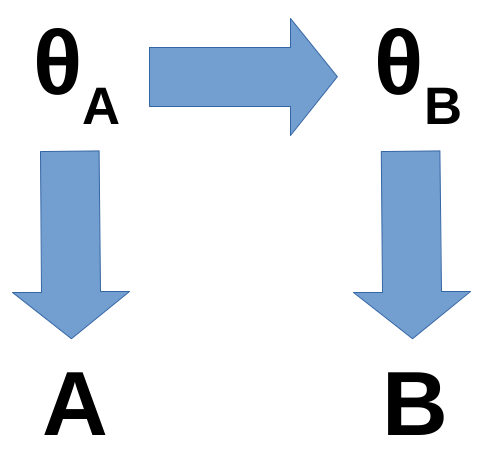
\includegraphics[width=.2\textwidth,keepaspectratio]{figs/transfer.png}
    
  
\item \textbf{Model Robustness: (e.g. Noise; Channel)}

    %% 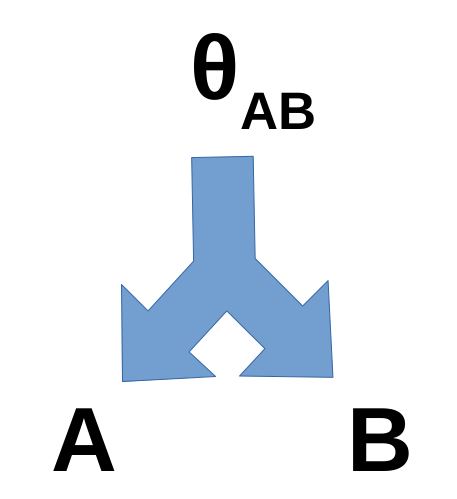
\includegraphics[width=.2\textwidth,keepaspectratio]{figs/robustness.png}
  
\end{itemize}



\newpage

\section{Experiments}

This section contains the main contributions of the dissertation research.

This dissertation investigates training methods for acoustic modeling in the Neural Net + HMM ASR pipeline.

I aim to produce acoustic models which perform better (i.e. lower Word Error Rates) on datasets which are not similar the original training dataset.

I investiage the effectiveness of different \texttt{Tasks} (eg. linguistic \texttt{Tasks} vs machine learning \texttt{Tasks}) in a Multi-task Learning framework.


\subsection{Data}

I am creating acoustic models which generalize well to new data. To measure how well the models generalize, I use a set of speech corpora which exhibit some interesting differences between training and testing data. These differences between corpora exemplify the typical challenges faced in speech recognition generalization.

The training and testing data will differ in either (1) the recording \texttt{noise} conditions, (2) who the \texttt{speaker} is, or (3) what \texttt{language} the speaker is using. The following table shows which data sets are used for each audio condition.


\begin{table}[!htbp]
  \centering
  \begin{adjustbox}{width=.75\textwidth}
    \begin{tabular}{clcc}
      \toprule
      && \multicolumn{2}{c}{\textsc{Corpus}}\\
      && \textbf{Train} & \textbf{Test}\\
      \midrule
      \multirow{3}{*}{\textsc{Audio Condition}} &\textbf{Noise} & TIDIGITS & Aurora 5 \\
      &\textbf{Speaker} & LibriSpeech-A & LibriSpeech-B \\
      &\textbf{Language} & LibriSpeech & Kyrgyz Audiobook \\
      \bottomrule
    \end{tabular}
    \label{table:data}
  \end{adjustbox}
  
  \caption{Speech Corpora}
  
\end{table}


\subsection{Model Training Procedure}

This dissertation investigates the creation of new tasks for MTL, either using (1) linguist-expert knowledge, (2) ASR Engineer-expert knowledge, or (3) general Machine Learning knowledge.

The former two knowledge sources are useful for buidling acoustic models, but not much else. On the other hand, the final knowledge source (general machine learning concepts) can be applied to \textit{any} classification problem.

The three knowledge sources will be abbreviated as such:
  
\begin{itemize}
\item  (\textsc{LING}) \textbf{Linguistic Knowledge} 
\item (\textsc{ASR}) \textbf{Traditional Speech Recognition Pipeline}
\item (\textsc{ML}) \textbf{General Machine Learning}
\end{itemize}


Each of these categories contains a wealth of ideas, but I will consolidate each into three experiments. With three experiments for each knowledge source, my dissertation will contain nine (9) experimental conditions (for each audio condition).

Specifically, I will use the following concepts to create new tasks to be used in MTL training:

\begin{table}[!htbp]
  \centering
  \begin{adjustbox}{width=.55\textwidth}
    \begin{tabular}{cccc}
      \toprule
      & \multicolumn{3}{c}{\textsc{Knowledge Source}}\\
      & \textbf{LING} & \textbf{ASR} & \textbf{ML}\\
      \midrule
      \multirow{3}{*}{\textsc{Experiments}} & voicing & monophones &  k-means \\
      & place & $1/2$ triphones & random forests  \\
      & manner & $3/4$ triphones &  bootstrapped resamples  \\
      \bottomrule
    \end{tabular}
    \label{table:data}
  \end{adjustbox}
  
  \caption{Experimental Setup}
  
\end{table}


Each of these tasks will be added to a Baseline model. More specifically, the Baseline model will be a Neural Net with a single output layer (Task A), and the tasks above will be added as a second task (Task B). You can think of the tasks as simply a new set of labels for the existing data set. For example, when the \textsc{Ling} task of \textsc{voicing} is used, any audio segment labeled \texttt{[b]} will be assigned the new label \texttt{voiced}.

When these experiments will be applied to each of the three audio conditions, we get the following 30 experiments:

\begin{table}[!htbp]
  \centering
  \begin{adjustbox}{width=.75\textwidth}
    \begin{tabular}{ccclc}
      \toprule
      \textbf{Data Condition} & \textbf{Train Data} & \textbf{Test Data} & \textbf{MTL Training Tasks} & \textbf{Num. Exps} \\
      \midrule
      \multirow{4}{*}{\textsc{Noise}} & \multirow{4}{*}{\textsc{TIDIGITS}} & \multirow{4}{*}{\textsc{Aurora 5}} & Basline & 1\\
      & & & Baseline + LING & 3   \\
      & & & Baseline + ASR  & 3  \\
      & & & Baseline + ML   & 3  \\
      \midrule
      \multirow{4}{*}{\textsc{Speaker}} & \multirow{4}{*}{\textsc{LibriSpeech-A}} & \multirow{4}{*}{\textsc{LibriSpeech-B}} & Baseline & 1 \\
      & & & Baseline + LING & 3  \\
      & & & Baseline + ASR  & 3  \\
      & & & Baseline + ML   & 3  \\     \midrule
      \multirow{4}{*}{\textsc{Language}} & & \multirow{4}{*}{\textsc{Kyrgyz-B}} & Baseline & 1\\
      & \textsc{LibriSpeech +} & & Baseline + LING  & 3 \\
      &  \textsc{Kyrgyz-A} & & Baseline + ASR   & 3 \\
      & & & Baseline + ML & 3 \\
      \midrule
      &&&& 30\\
      \bottomrule\\
    \end{tabular}
    \label{table:data}
  \end{adjustbox}
  
  \caption{Experimental Setup}
  
\end{table}


\subsection{Task Creation Specifics}


\begin{enumerate}

\item \textbf{Baseline}

All the following architectures will be compared to the performance of the following baseline.

To account for any advantage mutliple output layers may bring about, the baseline also contains two output layers, where the \texttt{Tasks} are identical. In this way, random initializations in the weights and biases for each \texttt{Task} are accounted for.

During testing, \textit{only one} of the \texttt{Tasks} is used. The additional \texttt{Tasks} are dropped and the \texttt{Baseline Triphones} are used in decoding. This highlights the purpose of the extra \texttt{Tasks}: to force the learning of robust representations in the hidden layers during training. The \texttt{Tasks} may in fact not be the best option for final classification; they serve as ``training wheels'' which are then removed once the net is ready. 

\begin{figure}[!htb]
  \centering
\minipage{0.33\textwidth}
  
\includegraphics[width=\linewidth]{figs/mtl-arch-baseline.png}
  \caption{\texttt{Baseline}}
\endminipage\hfill
\end{figure}



\item \textbf{LING}

  All of the linguistic knowledge tasks view the phoneme as a bundle of features.

  Using standard features from articulatory phonetics (voicing, place, and manner), the following tasks generate labels for each data point by collapsing the given phoneme labels along one of these three dimensions.

  All information from one dimension is removed from the labeled data. This forces the classifier to rely on audio signal features which do not relate to that dimension. The DNN must project the input data into a new space for classification, using only information from the other two dimensions. 

  
  \begin{enumerate}
  \item \textsc{voicing}

    Voicing information is removed from the data labels.

    Speaker Robustness Experiments: The training data is a 4.5 hour subset of Librispeech, with mixed speakers, men and women. The testing data is 30 minutes of speech from two speakers (one man one woman).

    First, two separate GMM-HMM models are trained on the training data. The first GMM-HMM model uses the standard CMUDict phoneset (39 phones + stress variants).


%% \begin{table}[!htbp]
%%   \centering
%%   \begin{adjustbox}{width=.5\textwidth}
%%     \begin{tabular}{lll}
%%       \toprule
%%       \textbf{Phoneme} & \textbf{Example} & \textbf{Translation} \\
%%       \midrule
%%       \texttt{AA} &	odd  &   AA D \\
%%       \texttt{AE} &	at &	AE T \\
%%       \texttt{AH} &	hut &	HH AH T \\ 
%%       \texttt{AO} &	ought &	AO T \\ 
%%       \texttt{AW} &	cow	 & K AW \\
%%       \texttt{AY} &	hide &	HH AY D \\
%%       \texttt{B} & 	be	& B IY \\
%%       \texttt{CH} &	cheese	& CH IY Z \\
%%       \texttt{D} & 	dee	& D IY \\
%%       \texttt{DH} &	thee	& DH IY \\
%%       \texttt{EH} &	Ed	& EH D \\
%%       \texttt{ER} &	hurt	& HH ER T \\
%%       \texttt{EY} &	ate	& EY T \\
%%       \texttt{F} & 	fee	& F IY \\
%%       \texttt{G} & 	green	& G R IY N \\
%%       \texttt{HH} &	he	& HH IY \\
%%       \texttt{IH} &	it	& IH T \\
%%       \texttt{IY} &	eat	& IY T \\
%%       \texttt{JH} &	gee	& JH IY \\
%%       \texttt{K} & 	key	& K IY \\
%%       \texttt{L} & 	lee	& L IY \\
%%       \texttt{M} & 	me	& M IY \\
%%       \texttt{N} & 	knee	& N IY \\
%%       \texttt{NG} &	ping	& P IH NG \\
%%       \texttt{OW} &	oat	& OW T \\
%%       \texttt{OY} &	toy	& T OY \\
%%       \texttt{P} & 	pee	& P IY \\
%%       \texttt{R} & 	read	& R IY D \\
%%       \texttt{S} & 	sea	& S IY \\
%%       \texttt{SH} &	she	& SH IY \\
%%       \texttt{T} & 	tea	& T IY \\
%%       \texttt{TH} &	theta	& TH EY T AH \\
%%       \texttt{UH} &	hood	& HH UH D \\
%%       \texttt{UW} &	two	& T UW \\
%%       \texttt{V} & 	vee	& V IY \\
%%       \texttt{W} &	we	& W IY \\
%%       \texttt{Y} &	yield	& Y IY L D \\
%%       \texttt{Z} &	zee	& Z IY \\
%%       \texttt{ZH} &	seizure	& S IY ZH ER \\
%%       \bottomrule
%%     \end{tabular}
%%     \label{table:data}
%%   \end{adjustbox}
%%   \caption{CMUDict Phoneset}
%% \end{table}


    From this standard phoneset, the normal 3-state monophones are trained from a flat-start via EM training. A total of XXX states are trained with a total of XXX Gaussian components over XXX iterations of EM. These monophones are then expanded into context-dependent triphones via a phonetic decision tree, with a maximum of XXX leaves. The resulting leaves (state clusters) are then trained with XXX Gaussian components over XXX iterations of EM. The final model acheives a WER of XXX on the testing data.

    The second GMM-HMM model trained differs from the first model in its set of initial phones. Instead of building monophones (and then triphones) from the standard CMUDict, this \texttt{-Voicing} model collapsed all voicing information from the phonetic dictionary (i.e. the lexicon file).


\begin{verbatim}
B P   --> P
CH JH --> CH
D T   --> T
DH TH --> TH
F V   --> F
G K   --> G
S Z   --> S
SH ZH --> SH
\end{verbatim}
    

    
  \item \textsc{place}

    All place information is removed from the data labels.

\begin{verbatim}  
F TH SH S HH --> F        voiceless fricatives
V DH Z ZH    --> V        voiced fricatives
P T K        --> P        voiceless plosives    
B D G        --> B        voiced plosives
M N NG       --> N        voiced nasal
L R          --> R        voiced laterals
Y W          --> Y        voiced approximants
\end{verbatim}      
 
  \item \textsc{manner}
    
    All manner information is removed from the data labels.

\begin{verbatim}
B M V W --> W          voiced labials
P F     --> P          voiceless labials
D Z     --> D          voiced alveolar
N L R   --> R          voiced alveolar2
T S     --> T          voiceless alveolar
ZH JH   --> JH         voiced postalveolar
SH CH   --> CH         voiceless postalveolar
NG G    --> G          voiced velar
\end{verbatim}

  \end{enumerate}


\begin{figure}[!htb]
\minipage{0.32\textwidth}
  
\includegraphics[width=\linewidth]{figs/mtl-arch-voicing.png}
  \caption{\texttt{-Voicing}}
\endminipage\hfill
\minipage{0.32\textwidth}
  
\includegraphics[width=\linewidth]{figs/mtl-arch-place.png}
  \caption{\texttt{-Place}}
\endminipage\hfill
\minipage{0.32\textwidth}%
  
\includegraphics[width=\linewidth]{figs/mtl-arch-manner.png}
  \caption{\texttt{-Manner}}
\endminipage
\end{figure}




\item \textbf{ASR}

  All the following tasks relate to the structure of the phonetic decision tree used in the traditional ASR pipeline to cluster context-dependent triphones. In GMM training the leaves of the decision tree are then assigned their own Gaussians, and in DNN training the same leaves are used as labels during training via backprop.

  The main intuition behind these experiments is that in using the decision tree labels as targets for the DNN classifier, we are performing model transfer. The decision tree and it's associated Gaussians perform classification, and we are merely training a DNN to perform that same task. So, the decision tree can be thought of as a single task for the DNN to learn.

  However, the DNN only sees the leaves of the decision tree. It doesn't see any of the branches, or any of its wonderful linguistic structure. So, in order to force the DNN to learn the information hidden in the decision tree, the following tasks are like cross-sections of the tree, slicing it from leaves up. The DNN then has to learn how to read these cross-sections, and how to map data onto each layer.

  If we slice the tree at the roots, we have the \textsc{monophones}. If we slice down half-way (\textsc{1/2 triphones}), we have more contextual information than monophones but less than full triphones. If go a little farther down (\textsc{3/4 triphones}), we get even more context, but less general information about the original phoneme.
  
  \begin{enumerate}
  \item monophones

    When we chop the tree at the roots.
    
  \item 1/2 triphones

    Chop the tree half-way down.
    
  \item 3/4 triphones

    Chopping a little further.
    
  \end{enumerate}


  

\begin{figure}[!htb]
\minipage{0.32\textwidth}
  
\includegraphics[width=\linewidth]{figs/mtl-arch-mono.png}
  \caption{\texttt{Monophones}}
\endminipage\hfill
\minipage{0.32\textwidth}
  
\includegraphics[width=\linewidth]{figs/mtl-arch-halfTri.png}
  \caption{\texttt{1/2 Triphones}}
\endminipage\hfill
\minipage{0.32\textwidth}%
  
\includegraphics[width=\linewidth]{figs/mtl-arch-3QuarterTri.png}
  \caption{\texttt{3/4 Triphones}}
\endminipage
\end{figure}



\item \textbf{ML}

  The following tasks do not make use of any linguistic knowledge or any part of the ASR pipeline. The only things needed to perform these tasks is labeled data.

  The two approaches above use linguistics or the ASR pipeline to force a DNN to learn structure about the data, because that information is useful for classification.

  We typically do not have this kind of \textit{a priori} information about the datasets we use in Machine Learning. Therefore, an interesting problem is how to learn this structure in a data set when we don't have access to that expert knowledge.

  The following tasks force the DNN to learn structure in the data without any knowledge about that structure. In order to do so, I make the assumption that the data does in fact have heirarchical relations. That is, I assume the \texttt{(data,label)} pairs were generated by something like a phonetic decision tree, and I try to recover the structure of that tree.
  
  \begin{enumerate}
  \item k-means

    Standard k-means on the data, with the caveat that labels cannot be split across clusters. A first round of clustering is performed, and then all data from the same original label are shifted to the cluster with the most data points from that label. Then, centroids are recalculated, and data is re-clustered. This adapated k-means should find related data points in the same clusters. If k-means is working, we would expect to be able to recover phonemes (monophones) from the labeled triphone data.
    
  \item random forest

    In another attempt to cluster triphones along phonetic categories, the random forest procedure works as follows: (1) take a random subset of the labels, (2) train a random forest with all data points associated with those labels, (3) re-classify all the rest of the data with the new random forest. In this way, we will reduce the number of labels (eg. out of 2,000 triphone labels I choose 500), and classify unseen data as its closest seen data point.

  \item bootstrapped resamples

    In this approach, new labels are not generated at all. The separate tasks for the DNN are just different samples of the data.

    Some sub-samples may exhibit a more useful decision plane than others, and if we randomly subsample for multiple tasks, the different decision planes will all have something in common. The individual peculiarities of one sub-sample will have to be ignored for the DNN to perform well on all tasks.
    
  \end{enumerate}

\begin{figure}[!htb]
\minipage{0.32\textwidth}
  
\includegraphics[width=\linewidth]{figs/mtl-arch-kMeans.png}
  \caption{\texttt{k-means}}
\endminipage\hfill
\minipage{0.32\textwidth}
  
\includegraphics[width=\linewidth]{figs/mtl-arch-forest.png}
  \caption{\texttt{1/2 Triphones}}
\endminipage\hfill
\minipage{0.32\textwidth}%
  
\includegraphics[width=\linewidth]{figs/mtl-arch-resampled.png}
  \caption{\texttt{3/4 Triphones}}
\endminipage
\end{figure}





\end{enumerate}








\end{document}





%% CMUDict: used for Librispeech

%% @article{davis1952automatic,
%%   title={Automatic recognition of spoken digits},
%%   author={Davis, KH and Biddulph, R and Balashek, Stephen},
%%   journal={The Journal of the Acoustical Society of America},
%%   volume={24},
%%   number={6},
%%   pages={637--642},
%%   year={1952},
%%   publisher={ASA}
%% }

%% @article{juang2005automatic,
%%   title={Automatic speech recognition--a brief history of the technology development},
%%   author={Juang, Biing-Hwang and Rabiner, Lawrence R},
%%   journal={Georgia Institute of Technology. Atlanta Rutgers University and the University of California. Santa Barbara},
%%   volume={1},
%%   pages={67},
%%   year={2005}
%% }


